
\section{OpenETCS Process}


\subsection{Overall Description}
\label{sec:overall_description}


To pursue the goals given in the introduction, the development cycle for the project is presented in this document.

In order to minimise the number of different models and unused steps, the proposed process shall take into account the safety concepts from the early steps, i.e., the sub-system requirement specification (SSRS) and the semi-formal definition of the model instead of the SRS. Thus, these elements can be used in the safety process to deduce formal models as shown in figure \ref{fig:OETCSProcess}.

The two most important elements of the System life-cycle of EN 50129 and the Software development life-cycle model of EN
50128 are the separation of the life-cycle into well-defined
phases and the focus on the production and recording of extensive documentation of the
development process. This allows facilitation of safety, verification, validation and assessment activities and confidence in the use of good practises to develop a critical system. To achieve this, an appropriate life-cycle
must be defined for OpenETCS, following the constraints provided by the CENELEC standard, and appropriate roles and responsibilities must be assigned to the participants.

 \begin{figure}
  \centering
  \fbox{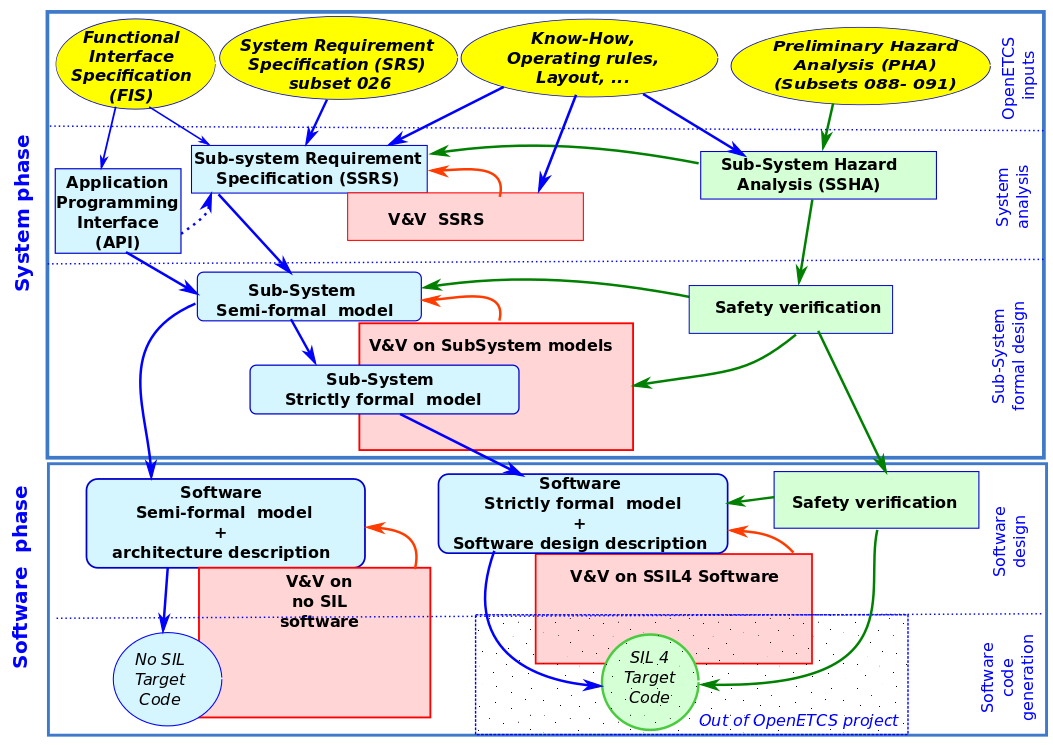
\includegraphics[scale=0.45]{WholeProcess.png}}
  \caption{Whole process}
  \label{fig:whole_process}
\end{figure}

Figure~\ref{fig:whole_process} described the main phases and main activities of the OpenETCS process.
Input elements of the project are in yellow, specification and design activities in blue, verification and validation activities in red, safety activities in green.

Two main phases are defined :
\begin{description}
\item[System phase] to analyse the input documents and provide a model of the on board unit according SUBSET-026 and safety strategy:
\begin{itemize}
\item First system analysis shall provide a \textit{Sub-System Requirement Specification} (SSRS) to define the scope of the system to  design and its structure, completed with an abstract \textit{Application Programming Interface} (API) to  give the main interfaces of the system and interaction between software and hardware items. \textit{Sub-System Hazard Analyses} (SSHA) allow the definition of safety properties.
\item Secondly, a model, at least semi-formal, is designed to  describe sub-system  architecture, main functions  and to allocate sub-system requirements. This model can be completed with a formal model to focus on some functions or properties.
\end{itemize}
\item[Software phase] to  design the software and then generate applicative code of the sub-system. Two  approaches are developed together from the same sub-system model:
\begin{itemize}
\item on one part to complete the semi-formal model to obtain a functional code covering as much as possible of the SSRS
\item on the other part to provide methods and tools to  obtain a SIL4 code and to apply this approach on a subset of the SSRS.
\end{itemize}
\end{description} 

In the sequel, the main lines of this figure are going to be detailed. However, we are going to focus on specification and design activities only.

The Software Planning phase is defined by WP1 in the Quality Assurance Plan.
The Software Test / Validation phase is defined by WP4 in the Validation Plan.
The Software Verification activities are defined by WP4 in the Verification Plan.

Safety activities are described in EN50126.
The proof that the process satisfies the requirements of the standard is out of the scope of this document and shall be managed by the Safety Case (WP4).



%%%%%%%%%%%%%%%%%%%%%%%%%%%%%%%%%%%%%%%%%%%%%%%%%%%%

\subsection{OpenETCS inputs}
\label{sec:inputs}

\tbd

The main input of the OpenETCS project is the SUBSET-026~3.3.0, which can be considered as the \emph{System Requirement Specification} (see R-WP2/D2.6-01-011).



However, this document is not sufficient to produce a model of the on-board unit software. Thus a \emph{Sub System Requirement Specification} shall be produced during this phase, in particular to define the structure of the system and to manage the requirement allocation (see R-WP2/D2.6-X-12).

External interfaces are partially provided by the UNISIG documents. However interfaces between ETCS units and application programming interfaces (API)  have to be defined for the OpenETCS project.



%%%%%%%%%%%%%%%%%%%%%%%%%%%%%%%%%%%%%%%%%%%%%%%%%%%%

\subsection{System Analysis}
\label{sec:sys-analysis}


\subsubsection{Objectives}
\label{sec:sys-ana-objective}

The aim of this phase is to have a clear definition of the sub-system to design, which is not given by the input documents, and to define the scope of the model to design. Thus during this step, we shall identify:

\begin{itemize}
\item a set of requirements which describe the functionalities of the sub-system and the expected results concerning performance, maintainability, safety, reliability,...
\item the description of the architecture of the sub-system
\item the description of the external and internal interfaces of the sub-system.
\end{itemize}

Safety activities are necessary to define the safety requirements of the system and to define which functions are considered vital or non-vital respectively.

\subsubsection{Outputs}
\label{sec:sys-ana-outputs}

According to  design activities, two documents shall be produced during this phase :

\begin{description}
\item[Sub-System Requirement Specification (SSRS)] shall define the scope and the structure of the sub-system and  manage the requirement allocation (see R-WP2/D2.6-X-10).
\item[Application Programming Interface (API)] shall describe the interfaces of the sub-system.
\end{description}


According the CENELEC standards, these documents complete the inputs document (SRS and FIS) to produce :
\begin{itemize}
\item the \emph{System  Requirements Specification} which describes all requirements of the system
\item the \emph{System Architecture Description
and Software / HW interface definition } which specify how the Software and the HW interact
as well as the location of the boundary between the two
\end{itemize}

\subsubsection{Detailed Description}
\label{sec:sys-ana-descr}

The first part is the definition of the  \emph{Sub System Requirement Specification} (SSRS) which shall allow:
\begin{itemize}
\item to clearly define the scope of SUBSET-026 to take into account for the design (only on-board functionalities are designed, track-side functionalities are out of the scope of the project) (see R-WP2/D2.6-X-10.2.4),
\item to define the interfaces of the system: external interfaces and software/hardware interfaces (see R-WP2/D2.6-X-10.2.5, R-WP2/D2.6-X-10.2.6),
\item to provide a functional architecture of the system with inputs and outputs of each function identified (see R-WP2/D2.6-X-10.2),
\item to allocate SRS requirements to each function (see R-WP2/D2.6-X-10.3),
\item to classify Safety versus Non-Safety items (functions, input/output, requirements, ...) from the safety analyses results (see R-WP2/D2.6-X-11),
\end{itemize}

However, the SSRS shall be compliant with the input documents of TSI (subset 26, FIS, ...) (see R-WP2/D2.6-X-10, R-WP2/D2.6-X-10.2.7 and R-WP2/D2.6-X-10.4)

It shall also facilitate safety, design, verification, validation and maintenance activities: full traceability between SRS and SSRS shall be provided (see R-WP2/D2.6-X-10.5).

Detection of inconsistencies or ambiguities in the input documents shall be discussed and tracked (see R-WP2/D2.6-X-10.6).

These tasks need some interactions with safety activities, for example to define safety tags on functions, requirements,...

The second part is the definition of the \textit{Application Programming Interface} (API)....

\tbd

\subsubsection{Means and tools}

The SSRS and API shall be described as documents.
However these documents shall be completed by a semi-formal model to describe the functional architecture of the on-board unit (see R-WP2/D2.6-X-10.2.2):

\begin{itemize}
\item to  define the scope of the application to design (see R-WP2/D2.6-X-10.2.4),
\item to split the main function of the system into independent functions (see R-WP2/D2.6-X-10.2.1),
\item to describe the data flow between functions (see R-WP2/D2.6-X-10.2.3),
\item to describe the abstract interfaces of the sub-system and its environment, with respect to the existing input documents (see R-WP2/D2.6-X-10.2.5 and R-WP2/D2.6-X-10.2.6),
\item to  support allocation of the requirement to  the function and data (see R-WP2/D2.6-X-10.3).
\end{itemize}

The requirements from the SRS are allocated toward the
functions of the SSRS (the architecture), possibly split and rewritten in order to restrict their scope to these
functions. They are also rewritten in order to match the objects named in
the architecture (in particular internal and external I/O). The requirements are provided in natural language
(even if the objects are unambiguously named).

In view of verification activities, traceability between SSRS and SRS shall be provided (see R-WP2/D2.6-X-10.5). In practice, interpretations, additions and omissions of requirements shall be tracked and justified (see R-WP2/D2.6-X-10.5.1 and R-WP2/D2.6-X-10.5.3), as well as exported requirements  (see R-WP2/D2.6-X-10.5.2).

According to  CENELEC standards, no specific constraints are given on the tools used during this step: textual and graphical editors, with syntax checker, are needed to  produce documents and model. Tools classified as T1 according EN50128 can be used.

%%%%%%%%%%%%%%%%%%%%%%%%%%%%%%%%%%%%%%%%%%%%%%%%%%%%

\subsection{Sub-System formal design}
\label{sec:subsyst-formal-design}



\subsubsection{Objectives}
\label{sec:sys-fm-objective}

The aim of this phase is to provide a model of the sub-system from the SSRS:

\begin{itemize}
\item to provide a semi-formal reference specification of the sub-system requirements
\item to lift ambiguities
\item to detect errors and inconsistencies.
\end{itemize}


\subsubsection{Outputs}
\label{sec:sys-fm-outputs}


The main output of this step is a \textit{semi-formal model of the sub-system}  covering the architecture, interface description and requirement allocation of the SSRS.

This semi-formal model can be completed with \textit{strictly formal models} to improve the understanding of the sub-system and to provide elements for verification and validation activities.

\subsubsection{Detailed Description}
\label{sec:sys-dev-deta-descr}


To cover the OpenETCS project objective  of formal models, a semi-formal model of the system  specification is defined from  the SSRS (see R-WP2/D2.6-X-12). This model shall reflect the architecture defined in SSRS (see R-WP2/D2.6-X-10.2.2). Requirements of the sub-system can be refined in a semi-formal means but the semi-formal model  shall be as consistent as possible with the SSRS level of abstraction (see R-WP2/D2.6-X-12.2), in particular choices concerning software architecture and design have not to be described at this level.
In practice, all the requirements of SSRS (see R-WP2/D2.6-X-12.2.1) and of the sub-system Hazard analysis (see R-WP2/D2.6-X-12.2.2) shall be covered by the semi-formal model.

Traceability between semi-formal model and SSRS shall be provided (see R-WP2/D2.6-X-12.2.5): interpretations, additions and omissions of requirements shall be tracked and justified (see R-WP2/D2.6-X-12.2.3), as well as exported requirements  (see R-WP2/D2.6-X-12.2.6).

This semi-formal model can be completed with strictly formal models to improve the understanding of some part of the sub-system (see R-WP2/D2.6-X-14) and to  provide elements for verification and validation activities especially concerning safety properties.

To facilitate safety activities, the safety relevant function should be as much as possible insulated from non safety relevant functions (see R-WP2/D2.6-X-17).


\subsubsection{Means and tools}

The means of description of the semi-formal model shall be understandable by domain experts (see R-WP2/D2.6-X-27), providing graphical  description (see R-WP2/D2.6-X-27.1).

The semi-formal model shall reflect the functional architecture defined in SSRS. In particular the language used to  design the semi-formal model shall allow it to be modular and extensible (see R-WP2/D2.6-X-15).

In view of validation activities, the means of description of the semi-formal model shall allow to execute or simulate it (see R-WP2/D2.6-X-33).

Parts of the subsystem shall be modelled strictly formally (see R-WP2/D2.6-X-14). This formal model shall be derived from the semi-formal one (see R-WP2/D2.6-X-14.2), as straightforward and automated as possible (see R-WP2/D2.6-X-14.4). Thus, the semi-formal model shall be designed (language and structure) in order to allow the design and validation of the strictly formal model (see R-WP2/D2.6-X-14.3); and to be easily translatable to other languages (see R-WP2/D2.6-X-30).
As for semi-formal model, strictly formal model shall be modular and extensible (see R-WP2/D2.6-X-16) and shall refine the modular design of the semi-formal model (see R-WP2/D2.6-X-16.1).


The expressiveness of the language used to design the semi-formal and formal models shall allow formalisation of the classical objects used in the description of a critical system (see R-WP2/D2.6-X-31 and R-WP2/D2.6-X-32):

\begin{itemize}
\item state machines
\item time-outs
\item truth tables
\item arithmetics
\item braking curves
\item logical statements
\item messages and fields
\end{itemize}


In view of safety activities, the languages used for the models shall allow a declarative and formal expression of the safety properties (see R-WP2/D2.6-X-28), understandable by domain expert (see R-WP2/D2.6-X-28.1). The modelled safety properties shall be validated on the semi-formal model by test and on the strictly formal model by proof (see R-WP2/D2.6-X-23). Logical properties can be added to simplify the models but shall be validated just as the properties (see R-WP2/D2.6-X-34).

All means of description used shall be standardized or at least documented in detailed (see R-WP2/D2.6-X-29). 

According to  CENELEC standards, no specific constraints are given on the tools used during this modelling step: textual and graphical editors, with syntax checker, are needed to  produce documents and model. Tools classified as T1 according EN50128 can be used.


%%%%%%%%%%%%%%%%%%%%%%%%%%%%%%%%%%%%%%%%%%%%%%%%%%%%

\subsection{Software design}
\label{sec:sw-design}

\subsubsection{Objectives:}
\label{sec:sw-req-objective}


In this phase, the system requirements shall be refined to take into account software constraints.

Two branches appear:
\begin{itemize}
\item  The aim of the first branch  is to  design all the functionalities of the SSRS to  produce a functional code, without SIL. As much as possible of the requirement of SSRS shall be covered at this phase.
\item the aim  of the second branch is to provide a method and a toolchain to produce a SIL 4 code. This approach has to be evaluated on a subset of the SSRS requirements.
\end{itemize}


\begin{figure}[h]
  \centering
  \fbox{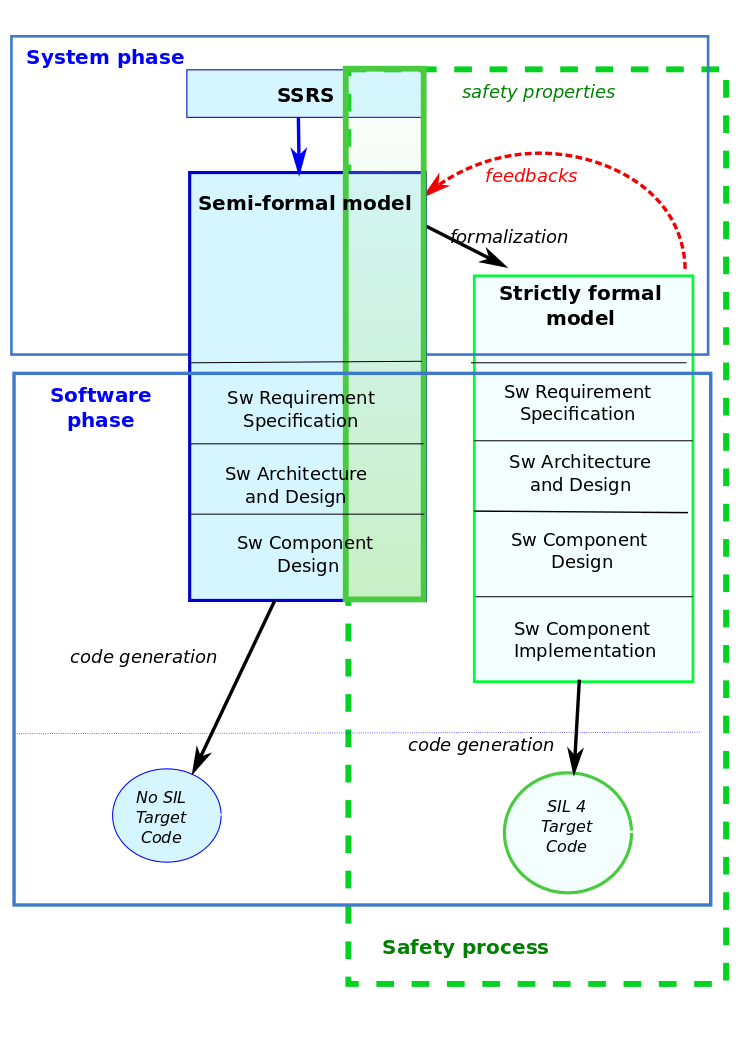
\includegraphics[width=4in]{Model-phase.png}}
  \caption{Software phase description}
  \label{fig:detailed software}
\end{figure}


\subsubsection{Functional branch}
\label{sec:sw-func}

For this branch, the semi-formal model  defined during the system phase, shall  be completed and detailed with software constraints, in such a way it is possible to produce an executable code for a given target.


\paragraph{Outputs:}
\label{sec:sw-func_out}

The main output of this step  is a semi-formal model which  allow to produce an executable code.
This model  shall be completed by a \textit{Software Architecture and Design Specification}, which describes the software architecture and the design choice.


\paragraph{Detailed Description:}
\label{sec:sw-req-deta-descr}

Taking into account the SSRS requirements allocated to  the software, a software architecture shall be defined, with a description of all the input/output of the software, as well as a description of the operational modes and behaviour.

Then, each software component is designed according to  the sub-system  requirements: All sub-system requirements, allocated to  software shall be referenced in the model or a justification shall be given.

It shall provide all the elements to have testable requirements on a target platform. All functions to perform shall be clearly identified. All existing constraints between hardware and software will be taken into account (cf. §7.2.1.1 of EN 50128).



 In this phase, there shall also be an evaluation of the
Hardware / Software interaction, its influence on the safety aspects of the system and the
evaluation of the usage of already existing Software. It shall also ensure the
testability and the appropriateness for formal proofs of the resulting Software, in
particular by minimising the complexity and the size of the safety relevant
parts (cf. §7.3.1.1 to 7.3.1.5 of EN 50128).

 Interfaces between software components and the software environment are described in the \emph{Software Interface Specification}.



\paragraph{Means and tools}
\label{sec:sw-means}

\begin{comment}
To be completed according requirement of EN50128  and D2.6
Use of formal methods to describe.
To each level shall be develop the semi-formal model ?

\end{comment}

\subsubsection{Functional and safety branch}


The model shall cover the three software development phases according EN 50128 :

\begin{itemize}
\item Software Requirements Phase
\item Software Architecture and Design Phase
\item Software Component Design Phase
\end{itemize}

\paragraph{Documents:}
\label{sec:sw-req-documents}
From a design point of view, the outputs to produce in this phase are:

\begin{itemize}
\item the Software Requirements Specification
\item the Software Architecture Specification
\item the Software Design Specification
\item the Software Interface Specification
\item the Software Component Design Specification
\end{itemize}



\paragraph{Detailed Description:}
\label{sec:sw-req-deta-descr}

The first step of this phase is to give an explicit description of software requirements according to system requirements and safety properties. The system architecture model from the preceding phase shall be
extended with a model of the software. All software requirements shall be referenced in that model.
In particular the \emph{Software Requirement Specification} shall give a description of all the input/output of the software, as well as a description of the operational modes and behaviour. It shall provide all the elements to have testable requirements on a target platform. All functions to perform shall be clearly identified. All existing constraints between hardware and software will be taken into account (cf. §7.2.1.1 of EN 50128).



Then, a \emph{Software Architecture Specification} shall be developed which allows meeting the software
requirements and the necessary safety requirements without introducing
unnecessary complexity. In this phase, there shall also be an evaluation of the
Hardware / Software interaction, its influence on the safety aspects of the system and the
evaluation of the usage of already existing Software. It shall also ensure the
testability and the appropriateness for formal proofs of the resulting Software, in
particular by minimising the complexity and the size of the safety relevant
parts (cf. §7.3.1.1 to 7.3.1.5 of EN 50128).

The \emph{Software Design Specification} shall give a  description of the design choices, in particular software component decomposition, data description and requirement allocations. Interfaces between software components and the software environment are described in the \emph{Software Interface Specification}.

Finally, the low level specification of each software components is defined in the \emph{Software
Component Design Specification} (cf. §7.4.1.1, §7.4.1.2 of EN 50128).

\paragraph{Means and tools}
\label{sec:sw-means}

\begin{comment}
To be completed according requirement of EN50128  and D2.6
Use of formal methods to describe.
To each level shall be develop the semi-formal model ?

\end{comment}

%%%%%%%%%%%%%%%%%%%%%%%%%%%%%%%%%%%%%%%%%%%%%%%%%%%%

\subsection{Software code generation}
\label{sec:sw-code}



\subsubsection{Objectives:}
\label{sec:sw-req-objective}


In this phase, the system requirements shall be refined to take into account software constraints.

Two branches appear:
\begin{itemize}
\item  The aim of the first branch  is to  design all the functionalities of the SSRS to  produce a functional code, without SIL. As much as possible of the requirement of SSRS shall be covered at this phase.
\item the aim  of the second branch is to provide a method and a toolchain to produce a SIL 4 code. This approach has to be evaluated on a subset of the SSRS requirements.
\end{itemize}




\subsection{Demonstrator}
\label{sec:demo-phase}


\paragraph{Objectives}
\label{sec:demo-objective}

\begin{comment}
What is the aim of the demonstrator ?  to provide an executable model of the on-board unit
What does that mean,
Which functionalities have to be taken into account ? Which are the interfaces and API ?
Does it take into account real-time, performance,... elements or just functional aspects ? What about safety ? What is the target platform ?
Non safety code ?
\end{comment}


\paragraph{Documents}
\label{sec:demo-documents}

\todo{input of the demonstrator : semi-formal model , at which level ?}


\paragraph{Detailed Description}
\label{sec:demo-deta-descr}


\begin{issue}
Manual versus automatic code generation ?
\end{issue}

\paragraph{Means and tools}
\label{sec:demo-means}

\todo{To detail according next meeting results}


%%%%%%%%%%%%%%%%%%%%

\subsection{Concrete Code}
\label{sec:code-phase}


\paragraph{Objectives}
\label{sec:code-objective}

This code cannot be provided by the OpenETCS project : Safety  activities are not conducted in the whole scope of the on-board unit subsystem, and elements of the target platform are not provided.

However, the description of how to  produce such a code in a safe way is part of the OpenETCS project. This corresponds to the lower phases of the process according to  E50128 :
\begin{itemize}
\item Software Component Implementation Phase
\item Integration
\end{itemize}


\paragraph{Documents}
\label{sec:code-documents}

According to EN50128, outputs of design for this phase are :
\begin{itemize}
\item  Software Source Code and supporting documentation
\end{itemize}


\paragraph{Detailed Description}
\label{sec:code-deta-descr}
\begin{issue}
Manual versus automatic code generation ?
\end{issue}

\todo{To detail according next meeting results}

\paragraph{Means and tools}
\label{sec:code-means}



\begin{comment}
Shall be replaced by automatic code generation from formal models using
refinement techniques.
\end{comment}


%%%%%%%%%%%%%%%%%%%%%%%%%%%%%%%%%%%%%%%%%%%%%%%%%%%%


